\chapter{Otros experimentos}
\label{appendix:otros}

\subsection{cnn}
Este estudio \cite{chentanez_cloth_2020} es un ejemplo de uso de CNN (redes convolucionales \footnote{Las redes neuronales convolucionales (CNN) son un tipo de arquitectura de DL diseñada para el procesamiento de datos estructurados en forma de cuadrícula, como imágenes, vídeos o secuencias temporales}), para la simulación de telas. Reseña la dificultad de intregar una CNN debido a la construcción de la malla, incompatible antes de su modificación con una cuadrícula 2D. Resuelve el problema entrenando mallas "manifold" triangulares: es decir, mallas cuyos bordes están conectados por al menos dos caras (menos los extremos) dejando una separación entre exterior e interior. Mapear la malla a una imagen 2D es lo que permite realizar la convolución.
Otro ejemplo de estudio que usa una CNN para la simulación de telas es DeepSD: Real-time Cloth Simulation with Deep Learning \cite{bertiche_deepsd_2021}; en la que proyecta la malla 3D en un plano utilizando sus coordenadas UV\footnote{Las UVs son coordenadas bidimensionales que definen cómo se proyecta una textura 2D sobre la superficie de un modelo 3D. El mapeo UV consiste en aplanar o desplegar una malla 3D sobre una superficie plana. }. Usa una CNN estándar, y no depende de una malla fija, pudiendo aceptar cambios en la topología de la malla, por lo que sirve para automatizar el proceso. El uso de SDF garantiza la generación de ropa que envuelva el cuerpo sin importar la concectividad de la malla durante los cálculos intermedios. No obstante, comparando con el estudio de  Chentanez et al. este estudio no consigue capturar arrugas finas o superficiales con detalle y es menos eficiente debido a su enfoque volumétrico. 



\subsection{anchored}
como similitud al skinned y la pose de reposo, 
\textbf{Anchored training:} Otra forma de intentar reducir el error consiste en inferir el desplazamiento de los vértices respecto a las posiciones originales de la malla en lugar de las posiciones en el último frame (\cite{bertiche_deepsd_2021}, \cite{santesteban2022snug}, \cite{holden_subspace_2019}). Este es un planteamiento intuitivo que se presenta en distintos papers mencionados previamente: DeePSD, SNUG o Subspace Neural Physics. Al pensar en simulaciones de telas, ya sea una bandera con su mástil o una prenda con su personaje, todas cuentan con unos puntos, es decir, algo a lo que anclarse. Actuando sobre esos puntos se puede asegurar que la simulación se mantendrá dentro de un espacio concreto. En esta investigación aplicamos esta técnica guardando las posiciones de los vértices en su estado incial y aplicando los nuevos desplazamientos sobre estos.
Al coger un punto de referencia del que medir los desplazamientos y no basarse en posicines generadas, el MSE del modelo, calculado como la diferencia entre las posiciones reales y predichas, en las pruebas de python mejora notablemente. No obstante, la simualción en Unity aún adolece de errores de pecisión.
        

\subsection{estático}
\begin{figure}[H]
	\centering
	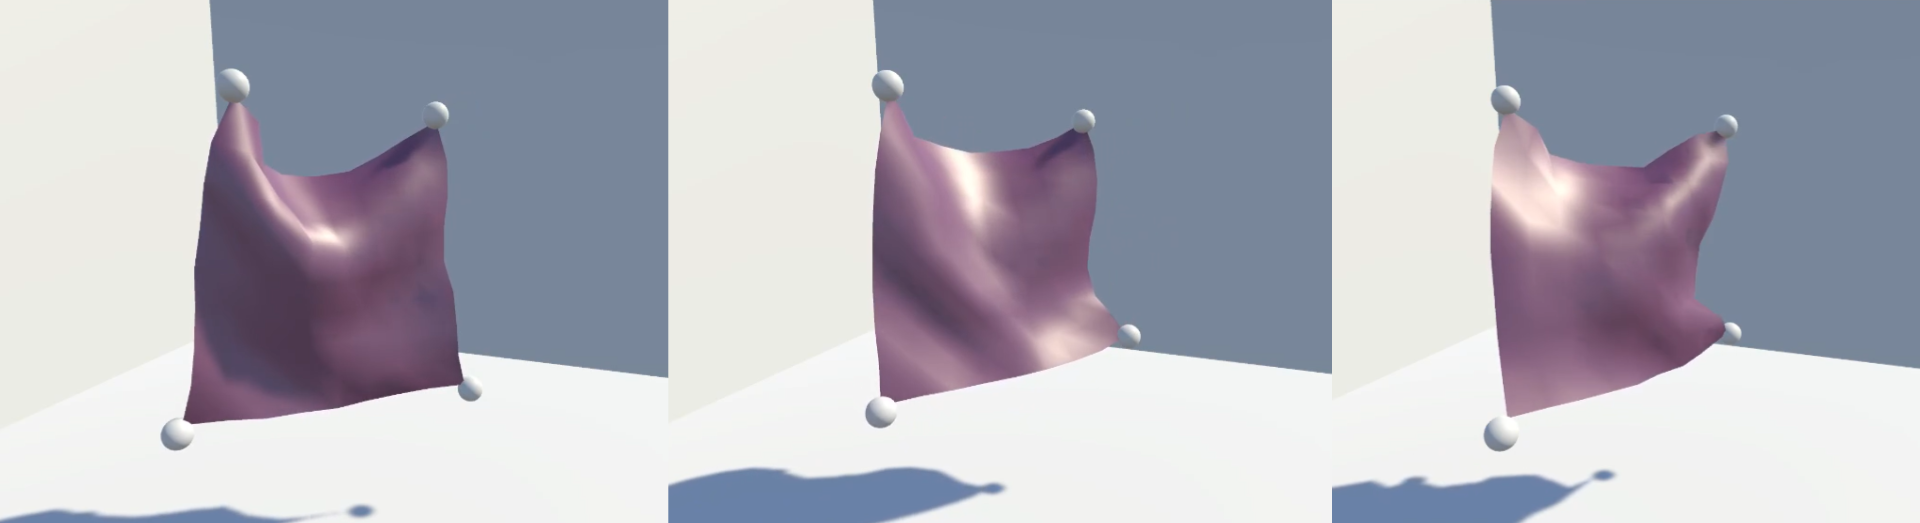
\includegraphics[width=0.8\textwidth]{Imagenes/estatico.png}
	\caption{Ejemplo de la simulación estática implementada.}
	\label{fig:arq}
\end{figure}